Almost all interpretability methods work on image classification tasks. To learn how these methods are applied, how they work and what output they generate, the first step in this work is applying these methods on a classification task. We chose a dataset from the medical imaging field: The NIH (National Institutes of Health, United States) chest X-ray dataset \cite{wang2017chestx}.

We downloaded the dataset, trained a neural network on the dataset and applied the selected methods described above.

\section{NIH Chest X-ray dataset}
The NIH Chest X-ray dataset contains 112,120 X-ray scans from 30,805 unique patients \cite{nihchestxraykaggle}. Every scan has one or more disease labels. Figure \ref{chest_xray_sample} show three sample images from the dataset.

\begin{figure}[h]
\centering
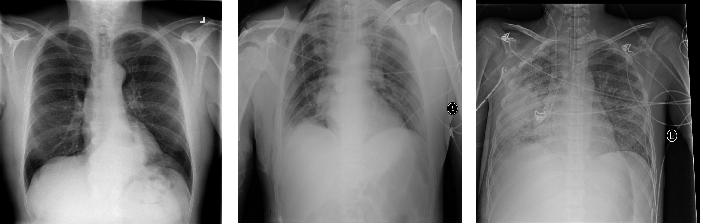
\includegraphics[width=14cm]{chapters/03_classification/images/chest-x-ray.png}
\caption{Examples for the NIH Chest X-ray dataset}
\label{chest_xray_sample}
\end{figure}

\section{Model Training}
We decided to train a model based on an existing neural network architecture, because building a state of the art architecture is very hard and not the focus of this thesis.

The detailed results of the training sessions are available in the results directory of the GitHub repository: \href{https://github.com/andef4/thesis-code/tree/master/nhs-chest-xray/results/}{nhs-chest-xray/results}.

\subsection{Inception ResNet v2}
\nblink{nhs-chest-xray/inception\_resnetv2.ipynb}

We chose Inception ResNet v2 \cite{szegedy2017inception} as the architecture. This is modern neural network built for image analysis and generally trained on the ImageNet dataset.
The ResNet variant of the Inception architecture delivers similar performance as the normal Inception model, but with significantly reduced training time.

\nblink{nhs-chest-xray/preprocess.ipynb}
The preprocessing steps required to use this architecture are resizing the images to 299x299 pixels and converting the gray-scale images to color images.
We also tried to modify the network to directly use gray-scale images, but this was not successful because the network architecture is built for three channel images.

We initially trained the network on a smaller subset (5607 image) of the dataset. The maximum reached validation accuracy was 40\%. The training times for the small training subset
were already very long, we therefore decided to abandon the Inception architecture for now and use a ResNet based architecture instead.

\subsection{ResNet}
\nblink{nhs-chest-xray/resnet.ipynb}

The first test of ResNet50 \cite{he2016deep} with pretrained parameters (trained on ImageNet) on the sample dataset showed fast training times but low accuracy. Training the network from scratch showed promising validation accuracy, which started to decrease on later epochs. The training accuracy was still increasing, this is therefore a clear indicator that the neural network is overfitting. We decided to change the architecture to ResNet18 which is a smaller ResNet variant with fewer parameters and should be less susceptible to overfitting.

The 

\begin{itemize}
    \item Epoch time of ~40 seconds instead of (TODO) 10 minutes/3 hours for full dataset
    \item resnet50 with pretrained
    \item resnet50 without pretrained
    \item resnet18 without pretrained
    \item resnet18 without pretrained full dataset
\end{itemize}




\subsection{Single label only}
65\%


\subsection{Only images with actual diagnosis}
https://www.kaggle.com/kmader/train-simple-xray-cnn 
For testing out the methods, images with findings are much more helpful, so filter them out.

Better results:

\subsection{Densenet}
\nblink{nhs-chest-xray/densenet.ipynb}



% https://medium.com/@jrzech/reproducing-chexnet-with-pytorch-695ff9c3bf66

Loading the saved model did not work, because the used version of PyTorch was old and incompatible with ours.

=> Retraining

\subsubsection{Image resize problems}
In the Densenet code there was a reference that some images were not properly resized. We did a short check on our preprocessed data, but it revelead no such problems. Used bash command:

\begin{minted}{bash}
find . -name '*.png' -exec file {} \; | cut -c 37-45 | uniq
\end{minted}

\subsection{Densenet single}
\nblink{nhs-chest-xray/densenet\_singleclass.ipynb}
\nblink{nhs-chest-xray/inception\_resnetv2\_singleclass.ipynb}

\begin{itemize}
    \item Fail: Not correctly setting up classes (last layer has 1000 classes for imagenet, we have 14)
    \item Fail 2: Train and validation set do not have same classes because of ordering in dataset loading code
\end{itemize}

After training for a short time with the fixes, we get an acceptable accuracy rate of 55\%. We then started to calculate the accuracy per class, as has been done on the reproduce-chexnet discussed above. We quickly discovered that only the "No findings" class was accurate, an all other classes had zero correct classifications.

\begin{itemize}
    \item test with no findings removed => not that better, finds only 3 classes correctly
    \item try with weighted cross entropy loss
\end{itemize}
